\section{ESIM Simulator and Event Camera Datasets}
\label{sec:esim_dataset}

Research on event cameras and event-based computer vision is still in its early stages. One of these reasons is tied to the hardware itself, since event cameras are expensive, not widely available, and are mostly prototypes, with low resolution (no more than 346x260 in the case of a state-of-the-art DAVIS346) and therefore not ready for commercial applications. Another such reason is the need for data and datasets, which are also scarce for the time being.
    
To tackle these problems, a number of simulators have been developed, of which ESIM (\cite{rebecq2018esim}) is an example, developed by Depts. Informatics and Neuroinformatics at ETH Zurich, in a similar spirit to the  conventional cameras simulator available. ESIM is an open-source ROS package.

\subsection{Simulators and ESIM}

Most event camera simulators continuously render images, and consecutive frames are compared. Events are then generated from big enough differences between frames.

A common problem with this technique is the choice of framerate, as a naïve approach would have the engine render at 1000 frames per second, in order to match the microsecond temporal resolution of event cameras. However, this is not ideal, as many frames are redundant, and therefore performance is affected. An ideal approach would only generate frames that are guaranteed to generate events, but at the same time should have a temporal resolution comparable to event cameras. ESIM uses a tightly coupled system between the simulator and the rendering engine, allowing for a better simulation, by using an adaptive sampling rate based on the dynamics of the scene.

Fig.\,\ref{fig:sec2_comparison_sampling} shows the advantage of an adaptive sampling approach as opposed to a uniform sampling approach. In the latter, rapid changes in the environment are sometimes overlooked.

\begin{figure}[ht]
    \centering
    \includegraphics[width = 1\linewidth]{comparison_sampling.PNG}
    \caption[Comparison of sampling approaches for the simulator]{Comparison of a uniform sampling approach (b) and an adaptive sampling approach (c) when recreating the reference response shown in (a), from \cite{rebecq2018esim}}
    \label{fig:sec2_comparison_sampling}
\end{figure}

 This adaptive sampling is possible due to a communication between the simulator itself, and the rendering engine being used. It relies on the knowledge of the trajectory of the virtual camera to estimate the motion on the scene, which is used to guess changes due to brightness, pixel displacement, noise and non-idealities, to adapt the sampling rate and the event generation. Fig.\,\ref{fig:sec2_esim_architecture} shows the ESIM architecture.

 \begin{figure}[ht]
    \centering
    \includegraphics[width = 1\linewidth]{esim_architecture.PNG}
    \caption[ESIM architecture]{Architecture of ESIM, showing the tight coupling between the simulator and rendering engine, sharing the information of time $t_k$, camera pose $T_{WC}(t_k)$ and camera twist $\xi(t_k)$, generating irradiance map $E(t_k)$ and motion field map $\nu (t_k)$, from \cite{rebecq2018esim}}
    \label{fig:sec2_esim_architecture}
\end{figure}

ESIM allows the use of multiple rendering engines and modes, such as as an OpenGL integration, as well as a photorealistic rendering using Unreal Engine. The simulation of stereo cameras, and panoramic cameras is also possible. Furthermore, it is possible to “convert” videos to events, though the results are not as good, due to the fixed sampling rate of the videos, and unusage of the rendering engine.

The generation of events is as previously described. This simulator also allows for the generation of images, in effect replicating the more advanced DAVIS event cameras. For the generation of frames, a simple capture of the render from the viewpoint of the camera is performed, at specific intervals, corresponding to the framerate of the camera being generated. It is also possible to simulate exposure time, producing images that are subject to motion blur (useful for a "fairer" comparison in high-speed motions).

The trajectory performed by the virtual camera is crucial for generating the sensor readings, in particular the IMU measurements (which include both accelerometer and gyroscope readings), as well as groundtruth trajectory values (for posterior validation of methods). An explanation of the type of information provided by IMUs is included in Section\,\ref{sec:sec2_imu}.

The simulator can generate a random trajectory, by defining a random set of points, and can also receive a trajectory predefined in a file. In both cases, the points being supplied are only indicative, and internally the simulator fits a spline to the trajectory. This concept is shown in Fig.\,\ref{fig:sec2_traj_sup_ob}, and is crucial to generate a smooth trajectory that can be continuously differentiable (notice the jagged trajectory supplied and the smooth trajectory received, shown in Fig.\,\ref{fig:sec2_traj_sup_ob}). 

\begin{figure}[ht]
	\centering
		\begin{tabular}{cc}
		   \includegraphics[width=0.45\linewidth]{supplied.eps} &
		   \hspace{1cm} \includegraphics[width=0.45\linewidth]{obtained.eps} \\
		   (a) & (b)  \\
		\end{tabular}
	\caption[Trajectory obtained through simulator and provided trajectory]{Comparison of the trajectory that was supplied to the simulator (a) vs. the trajectory that was performed by the simulator (b), and provided in the trajectory groundtruth. The trajectory corresponds to a movement in a single axis, back and forth}
	\label{fig:sec2_traj_sup_ob}
\end{figure}


The importance of the smooth trajectory is that it can be directly related to the sensor readings. Taking the accelerometer, for example, it measures the linear acceleration of the camera in space. Well, the acceleration of a body can be given as the second derivative of movement (the first derivative being velocity). Likewise, velocity and position can be obtained (apart from a constant) by integrating the acceleration. 

As a result of a the smooth trajectory from the spline, which is continuously differentiable, we can obtain the accelerometer reading for that axis by deriving the trajectory twice, as shown in Fig.\,\ref{fig:sec2_comp_imu}, which compares the accelerometer reading obtained by differentiating the trajectory twice, and the reading that was in fact generated by the simulator. It is possible to observe they coincide, apart from a slight noise and bias that the simulator generates in order to generate more realistic data.

\begin{figure}[ht]
	\centering
		\begin{tabular}{cc}
		   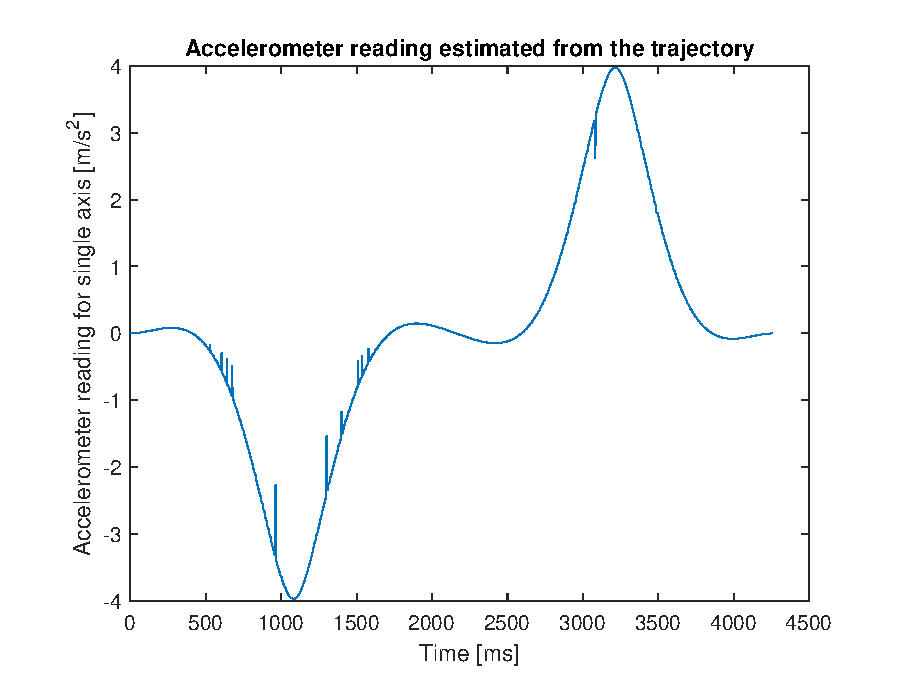
\includegraphics[width=0.45\linewidth]{acc_est.eps} &
		   \hspace{1cm} 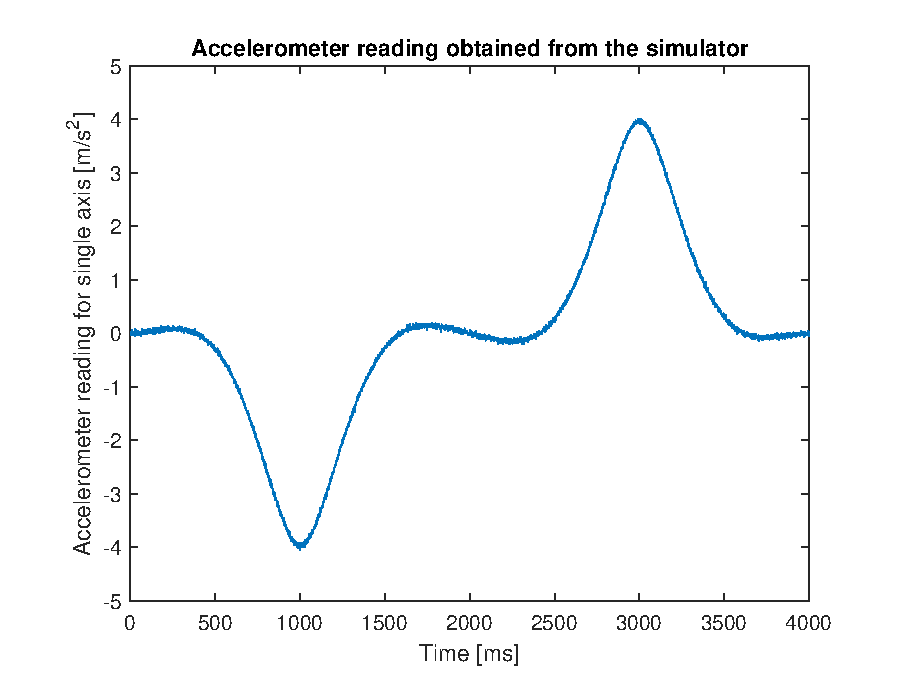
\includegraphics[width=0.45\linewidth]{acc_sim.eps} \\
		   (a) & (b)  \\
		\end{tabular}
	\caption[Comparison of sensor readings provided by simulator and the second derivative of the trajectory]{Comparison of the accelerometer reading obtained by differentiating the trajectory twice (a) vs. accelerometer reading that was obtained from the simulator (b). Notice the simulator adds some noise to simulate a real sensor. The spikes in (a) result from the discrete approximation of the derivative, but are not relevant for the relevance of the point being made and the comparison.}
	\label{fig:sec2_comp_imu}
\end{figure}

Likewise, for the other sensor readings (namely gyroscope), a similar approach is used, but instead taking the first derivative of the rotation along the trajectory.


\subsection{Datasets}

Datasets, like simulators, provide an interesting way to test algorithms without the need for a camera, compare results with other algorithms, and have a ground truth with which to benchmark.

The Depts. Informatics and Neuroinformatics at ETH Zurich provides a set of event camera datasets, recorded with a DAVIS 240C (an event camera with both events and full frames), along with IMU measurements and ground truth  (position and orientation) from a motion-capture system. Some of these datasets were used to test the algorithms developed.

Also, artificial datasets were generated through ESim, also to validate the algorithms developed with an accurate groundtruth.

%The datasets I have used are shapes_6dof.bag, which contains footage from a DAVIS240 of a collection of geometric shapes on a wall, and boxes_6dof.bag, which contains footage from a DAVIS240 of multiple boxes, with a complex texture.
